\subsubsection{Przygotowanie}
Skrypt rozpoczyna się od przygotowania środowiska do trenowania modelu.
Najpierw ustawia ścieżki do katalogów z wygenerowanymi grafami oraz do katalogów na dane treningowe i walidacyjne.
Następnie sprawdza, czy te katalogi istnieją, a jeśli nie, tworzy je.
Dalej, definiuje parametry dotyczące wielkości obrazów oraz wielkości partii danych, które będą używane podczas treningu.
Dla każdej wartości liczby wierzchołków ustawia ścieżkę do katalogu z wygenerowanymi grafami,
pobiera listę podkatalogów oraz obrazów w każdym z nich,
a następnie dzieli obrazy na zestawy treningowe i walidacyjne w stosunku 80:20.
Tworzy odpowiednie katalogi dla tych zestawów, jeśli jeszcze nie istnieją,
i kopiuje obrazy do właściwych lokalizacji, segregując je na treningowe i walidacyjne.

\subsubsection{Model}
Na początku dane zostały przygotowane ze zbioru obrazów, znajdującego się w katalogu lokalnym.
Dokonany został podział na zbiory treningowe i walidacyjne.
Dla każdego przejścia walidacji krzyżowej, dane zostały podzielone inaczej.
Po wczytaniu danych, zostały przeskalowane i przekształcone do odcieni szarości.

\begin{lstlisting}[language=Python,caption=Listing jedenego ze skryptów tworzących model,label={tests-model-1}]
	n_splits = 5
	kfold = KFold(n_splits=n_splits, shuffle=True, random_state=42)
	history = []
	all_images = [os.path.join(dp, f) for dp, dn, filenames in os.walk(data_dir) for f in filenames if os.path.splitext(f)[1] == '.png']

	for train_index, val_index in kfold.split(all_images):
		train_images = [all_images[i] for i in train_index]
		validation_images = [all_images[i] for i in val_index]

		# Dane treningowe
		train_ds = tf.keras.preprocessing.image_dataset_from_directory(
			data_dir,
			labels='inferred',
			label_mode='int',
			image_size=(img_height, img_width),
			batch_size=batch_size)
		class_names = train_ds.class_names
		train_ds = train_ds.map(lambda x, y: (rgb_to_grayscale(x), y))

		# Dane walidacyjne
		val_ds = tf.keras.preprocessing.image_dataset_from_directory(
			data_dir,
			labels='inferred',
			label_mode='int',
			image_size=(img_height, img_width),
			batch_size=batch_size)
		val_ds = val_ds.map(lambda x, y: (rgb_to_grayscale(x), y))

		# Model
		model = tf.keras.models.Sequential([
			tf.keras.layers.Rescaling(1./255),
			tf.keras.layers.Conv2D(32, 3, activation='relu'),
			tf.keras.layers.MaxPooling2D(),
			tf.keras.layers.Conv2D(32, 3, activation='relu'),
			tf.keras.layers.MaxPooling2D(),
			tf.keras.layers.Conv2D(32, 3, activation='relu'),
			tf.keras.layers.MaxPooling2D(),
			tf.keras.layers.Flatten(),
			tf.keras.layers.Dense(128, activation='relu', kernel_regularizer=tf.keras.regularizers.l2(0.01)),
			tf.keras.layers.Dropout(0.2),
			tf.keras.layers.Dense(len(class_names))
		])

		# Kompilacja modelu
		model.compile(
			optimizer='adam',
			loss=tf.losses.SparseCategoricalCrossentropy(from_logits=True),
			metrics=['accuracy']
		)

		# Uczenie modelu
		history.append(model.fit(
			train_ds,
			validation_data=val_ds,
			epochs=75
		))
\end{lstlisting}

Model sieci neuronowej został zdefiniowany jako sekwencyjny stos warstw.
Pierwsza warstwa to warstwa Rescaling, która normalizuje wartości pikseli do zakresu [0, 1].
Następne trzy warstwy to Conv2D z wybraną liczbą filtrów, z których każda jest poprzedzona warstwą MaxPooling2D.
Warstwy konwolucyjne używają różnych funkcji akytwacji, np. ReLU.
Po warstwach konwolucyjnych znajduje się warstwa Flatten, która przekształca mapy cech 2D w wektor 1D.
Następnie dodana jest w pełni połączona (Dense) warstwa z wybraną liczbą jednostek
i wybraną funkcją aktywacji, wraz z warstwą dropout.
Zastosowana jest tam również regularyzacja L2 (zmniejszanie wag) z ustaloną siłą regularyzacji wynoszącą.
Warstwa wyjściowa zawiera tyle jednostek, ile występuje klas.
Zależnie od danego testu, może być to różna liczba.

Dla standaryzacji danego testu ustalono K-Fold z liczbą podziałów równą 5.
Dla wszystkich warstw wybrana została funkcja aktywacji ReLU.
Liczba epok wyniosła 75.
W przypadku warstw konwolucyjnych, wybrano 32 filtry, a dla warstwy w pełni połączonej zastosowano 128 jednostek.
Regularyzacja została zastosowana z siłą 0,01, a współczynnik dropout - 0,2.

\subsubsection{Wyniki}
Po wytrenowaniu modelu, skrypt dokonuje wizualizacji dokładności i straty modelu w następujących krokach.
Najpierw wyświetla w konsoli wartości dokładności dla obu zbiorów z historii treningu.
Dalej tworzy wykresy, gdzie na pierwszym z nich pokazuje dokładność na zbiorze treningowym i walidacyjnym,
a na drugim wykresie prezentuje stratę modelu dla obu zbiorów.

\begin{figure}[ht]
	\centering
	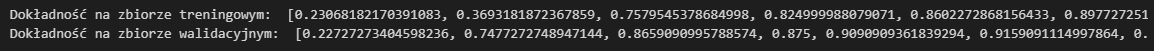
\includegraphics[width=15cm]{partials/tests/images/standard-result.png}
	\caption{Przykładowe wartości dokładności dla zbioru treningowe i walidacyjnego}
	\label{Fig:tests-wyniki-2}
\end{figure}
\FloatBarrier

\begin{figure}[ht]
	\centering
	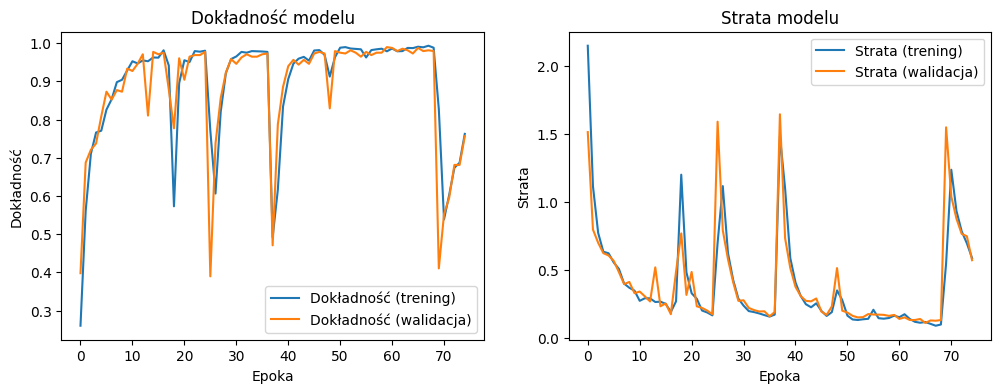
\includegraphics[height=5.5cm]{partials/tests/images/v2_epoch75.png}
	\caption{Przykładowa wizualizacja dokładności i straty wytrenowanego modelu}
	\label{Fig:tests-wyniki-1}
\end{figure}
\FloatBarrier

\subsubsection{Testy na danych zewnętrznych}
Po wyświetleniu dokładnosci modelu skrypt przeszukuje katalog z danymi i jego podkatalogi, by przygotować obrazy zewnętrzne.
Następnie ustawia ścieżkę do katalogu z obrazami testowymi i pobiera ich listę.
Dla każdego obrazu w tej liście wczytuje go, przeskalowuje do odpowiedniego rozmiaru i konwertuje do skali szarości
Następnie model przewiduje klasę obrazu, a wynik jest wyświetlany w konsoli.